%Nilocwords: 
% - Introduce ZigBee by first talking about its role in our project
% - Explain XBee / ZigBee relationship and differences.
\section{ZigBee}
\frame{\frametitle{ZigBee Overview}
	\begin{itemize}
		\item All inter-Satellite ("Mesh") communication
		\item Different than XBee:
			\begin{itemize}
				\item XBee is a small digital radio (Hardware)
				\item ZigBee is the specification it talks over ('Protocol')
			\end{itemize}				
	\end{itemize}
}

% - Compare specification to Bluetooth (relatable)
% - Low power, low data rate communication over digi radios
% - Explain PAN standard and why it's important
% - Explaining 'slightly' open source:
%		Open source as far as documentation and development,
%		however to be branded "ZigBee Compliant", must be member
%		of ZigBee Alliance. Has membership fee. Thus, conflicts
%		with GNU General Pub License
\subsection{What is ZigBee?}
\frame{\frametitle{What is ZigBee?}
	\begin{itemize}
		\item Specification, much like Bluetooth
		\item Low power communication over digital radios
		\item Based on 802.15.4 (PAN standard)
		\item 'Slightly' open-source
	\end{itemize}
}

% - ZigBee forms Mesh network on it's own
% 		save for some configurations in hardware
% - Explain how each feature is important to the project:
% 		Mesh is localized and encrypted (secure),
%		meaning Satellites can be safely added
%		in the target residence, quick and easy
% - Explain how ZigBee compliant devices 'bark' to each other
% 		and how adding nodes to the network expands the network's
%		effective range
\subsection{Why ZigBee?}
\frame{\frametitle{Why ZigBee?}
	\begin{itemize}
		\item Ad-hoc 'Mesh' networking
		\item Capable of adding nodes on-the-fly
		\item Localized and yet expandable network
		\item Has it's own encryption
	\end{itemize}
}

% - Any ZigBee Mesh has only one Coordinator,
%		which administrates and maintains Mesh.
% - Routers can send/rcv data for themselves,
%		and also route data to/from other ZigBee devices
% - End devices are super low-power, but require a
%		specific Router to be their 'parent.'
%		We aren't using these at all.
% - Explain massive amounts of radios per network
\subsection{How ZigBee Works}
\frame{\frametitle{How ZigBee Works}
	\begin{itemize}
		\item Three 'roles' in ZigBee networks:
		\begin{itemize}
			\item Coordinator
			\item Routers
			\item End-devices
		\end{itemize}
		\item Addressing scheme supports 
		\item Supports many network topologies
	\end{itemize}
}


% - Network types supported:
		Pair, Star, not very interesting.
%		Mesh is what we're using.
\subsection{Network Topology Examples}
\frame{\frametitle{Network Topology Examples}
\begin{figure}
\centering
%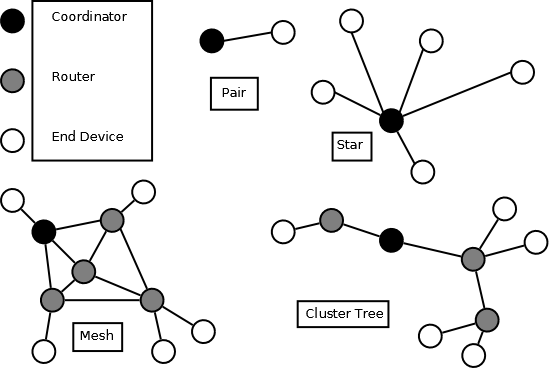
\includegraphics[scale=.8]{Diagrams/ZigBeeNetworkTypes.png}
\end{figure}
}